\documentclass[11pt,a4paper]{article}
\usepackage[T1]{fontenc}
\usepackage[utf8]{inputenc}
\usepackage{lmodern}
\usepackage[a4paper,margin=25mm,headheight=15pt]{geometry}
\usepackage{microtype}
\usepackage{amsmath,amssymb}
\usepackage[table]{xcolor}
\usepackage{booktabs,longtable,array,tabularx}
\usepackage{enumitem}
\usepackage{listings}
\usepackage{fancyhdr}
\usepackage{titlesec}
\usepackage{needspace}
\usepackage{etoolbox}
\usepackage{tikz}
\usetikzlibrary{arrows.meta,positioning}
\usepackage{hyperref}
\definecolor{navy}{HTML}{1F2A44}
\definecolor{blue}{HTML}{2D6CDF}
\definecolor{teal}{HTML}{0E7C7B}
\definecolor{muted}{HTML}{5B6472}
\definecolor{pale}{HTML}{F2F5F9}
\hypersetup{colorlinks=true,linkcolor=blue,urlcolor=teal,citecolor=teal,
 pdftitle={Achernar v5: System Architecture and Compute-Aware Local Model Runtime},
 pdfauthor={Ibrahim Shahid},pdfsubject={Architecture design; implementation status and validation requirements}}
\pagestyle{fancy}
\fancyhf{}
\lhead{\small\textcolor{muted}{Achernar / System Architecture v5}}
\rhead{\small\textcolor{muted}{October 3, 2026}}
\lfoot{\small\textcolor{muted}{Design specification / implementation status explicitly marked}}
\rfoot{\small\thepage}
\titleformat{\section}{\Large\bfseries\color{navy}}{\thesection}{0.65em}{}
\titleformat{\subsection}{\large\bfseries\color{blue}}{\thesubsection}{0.65em}{}
\titleformat{\subsubsection}{\normalsize\bfseries\color{teal}}{\thesubsubsection}{0.65em}{}
\pretocmd{\section}{\Needspace{12\baselineskip}}{}{}
\setcounter{tocdepth}{2}
\setcounter{secnumdepth}{3}
\setlength{\parindent}{0pt}
\setlength{\parskip}{6pt}
\setlength{\emergencystretch}{2em}
\setlist{nosep,leftmargin=1.5em,topsep=5pt}
\renewcommand{\arraystretch}{1.2}
\newcolumntype{L}[1]{>{\raggedright\arraybackslash}p{#1}}
\newcommand{\code}[1]{\texttt{\detokenize{#1}}}
\newcommand{\pathref}[1]{\texttt{\path{#1}}}
\newcommand{\current}{\textbf{Current implementation.}\ }
\newcommand{\planned}{\textbf{v5 requirement; implementation pending.}\ }
\lstset{basicstyle=\ttfamily\small,backgroundcolor=\color{pale},
 frame=single,rulecolor=\color{pale},breaklines=true,breakatwhitespace=false,
 columns=fullflexible,keepspaces=true,showstringspaces=false,tabsize=2,
 aboveskip=8pt,belowskip=8pt,xleftmargin=4pt,xrightmargin=4pt}

\begin{document}
\hypersetup{pageanchor=false}
\begin{titlepage}
\vspace*{14mm}
{\color{navy}\rule{\linewidth}{1.5pt}}\par
{\Huge\bfseries\color{navy} Achernar}\par
\vspace{5mm}
{\LARGE Unified Astronomy Imaging\\and Control System}\par
\vspace{8mm}
{\Large\color{blue} System Architecture v5}\par
{\large Compute-Aware Local Model Runtime,\\AI/ML Design, and Bounded Autonomous Control}\par
\vspace{12mm}
\begin{tabular}{@{}ll@{}}
Author & Ibrahim Shahid, Lead Architect\\
Revision date & October 3, 2026\\
Status & Accepted design direction; runtime implementation pending\\
Editable source & \code{achernar_v5.tex}\\
Historical baseline & \code{achernar_v4.pdf}, revised March 2026
\end{tabular}
\vfill
\textbf{Purpose}\par
Achernar should use the strongest validated perception model that a local
machine can execute reliably within its operational budget. Small models form
the minimum deployment tier. More capable hardware can qualify higher-capacity
variants without changing the physical meaning of observations or the authority
of the control and safety layers.
\vspace{5mm}
\textcolor{muted}{This is an edited architectural restatement of v4, reconciled
with the repository and the compute-aware runtime assessment. It is not a
byte-for-byte recovery of the unavailable v4 LaTeX source. Proposed APIs,
configuration, model tiers, and hardware support are identified as design work;
this document does not certify implementation or measured performance.}
\end{titlepage}
\pagenumbering{roman}
\hypersetup{pageanchor=true}
\tableofcontents
\clearpage
\pagenumbering{arabic}

\section{Executive Summary}
\label{sec:summary}
Achernar combines an on-site Rust daemon, a React operator interface, a Tauri
desktop shell, and a Django cloud platform. Hardware access, local acquisition,
measurement, and safety decisions belong to the daemon. Cloud services support
archiving, coordination, training, and analysis where implemented. The local
observing path must remain useful without a network connection.

The central v5 change is a compute-aware runtime for scalable perception.
The runtime inventories installed artifacts, identifies the execution providers
available in its build, validates deployed behavior, benchmarks eligible
candidates, and chooses a qualified implementation for each model family.
Hardware discovery supplies an initial prior; quality evidence and measured
resource constraints determine the selection.

\subsection{Scope and design status}
The words \emph{must} and \emph{shall} in proposed sections specify acceptance
requirements for future implementation. They do not imply that a module,
endpoint, or trained model already exists. Current behavior is grounded in the
working repository as inspected on the revision date. Dated audits remain
historical records, and the source code and migrations determine the current
executable contract.

\begin{longtable}{@{}L{0.23\linewidth}L{0.70\linewidth}@{}}
\toprule Area & Status at this revision\\\midrule\endhead
Classical vision & Implemented HFR, background, source rejection, and trailing
measurements. Unknown physical quantities remain unavailable where they cannot
be measured honestly.\\
FQE inference & Implemented optional shadow ONNX path, 64-pixel star crops,
batched execution, robust pooling, and hash-bound calibration. No accelerator
provider is configured by this path.\\
Shipped FQE artifact & Random reference graph for integration testing;
\code{runtime_eligible=false}. It is not a production model.\\
COC and TED neural paths & Metadata/placeholders exist; the runtime uses
heuristic/classical behavior. No trained production ONNX artifacts ship.\\
Focus drift & Implemented three-state Kalman estimator, with advisory output
and per-rig mutable state. It is not an ONNX network.\\
Generic model runtime & Registry scaffolding is not wired into startup;
generic ONNX runner is unfinished. Variant selection, provider qualification,
benchmark cache, and runtime status endpoints are proposed.\\
Accelerator releases & CUDA/TensorRT, CoreML, DirectML, and OpenVINO are
candidate deployment paths, not a validated support matrix.\\
\bottomrule
\end{longtable}

\subsection{Target users and deployment principle}
The same daemon architecture serves field equipment, backyard rigs, personal
laptops, and observatory workstations. A computer with more available compute
may qualify a larger or higher-resolution perception model. Executing unchanged
weights faster does not improve those weights' prediction quality. Additional
quality must come from a trained and validated variant, additional useful
observations, or a validated ensemble.

\section{System Architecture Overview}
\label{sec:architecture}
\subsection{Architecture layers}
The equipment layer contains cameras, mounts, focusers, wheels, and sensors.
The daemon owns device connections, acquisition, local storage, shared
perception, arbitration, and control. The client layer displays authoritative
daemon state and sends commands through a documented transport. The cloud
layer provides remote coordination and optional data services. External weather,
catalog, and astrometric resources require explicit freshness and availability
handling.

\begin{center}
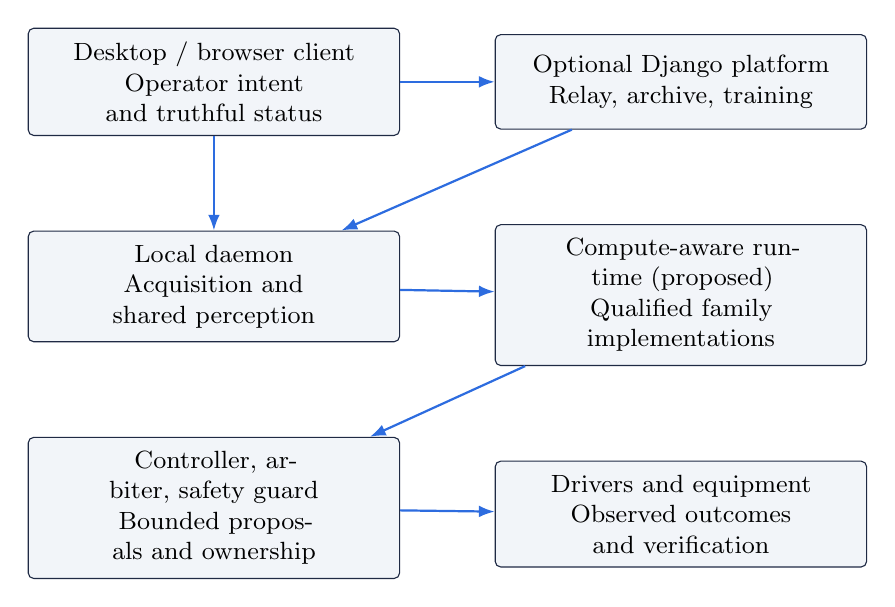
\begin{tikzpicture}[font=\small,
 box/.style={draw=navy,rounded corners=2pt,fill=pale,align=center,
 text width=0.36\linewidth,minimum height=12mm,inner sep=5pt},
 arrow/.style={-{Latex[length=2mm]},thick,blue}]
\node[box] (client) {Desktop / browser client\\Operator intent and truthful status};
\node[box,right=12mm of client] (cloud) {Optional Django platform\\Relay, archive, training};
\node[box,below=12mm of client] (daemon) {Local daemon\\Acquisition and shared perception};
\node[box,below=12mm of cloud] (runtime) {Compute-aware runtime (proposed)\\Qualified family implementations};
\node[box,below=12mm of daemon] (control) {Controller, arbiter, safety guard\\Bounded proposals and ownership};
\node[box,below=12mm of runtime] (equipment) {Drivers and equipment\\Observed outcomes and verification};
\draw[arrow] (client) -- (daemon);
\draw[arrow] (client) -- (cloud);
\draw[arrow] (cloud) -- (daemon);
\draw[arrow] (daemon) -- (runtime);
\draw[arrow] (runtime) -- (control);
\draw[arrow] (control) -- (equipment);
\end{tikzpicture}
\end{center}
The drawing shows responsibilities, not independent authority. A model runtime
never sends motor, exposure, filter, or mount commands. A larger model supplies
a potentially better estimate through the same family contract.

\subsection{One product, several qualified deployments}
Perception families can use different tiers on one machine. For example, FQE
may run a larger network while COC remains on a small network and the background
estimator remains classical. Per-family selection is subject to a joint resource
budget: qualifying each family in isolation is insufficient if their simultaneous
memory or compute demand exceeds the observing budget.

\section{Equipment Layer}
\subsection{Capabilities and hardware qualification}
The design retains the v4 camera, mount, focuser, filter-wheel, and environmental
sensor categories, including OLS/vendor SDK paths, Alpaca, and planned INDI or
direct interfaces. A declared Rust driver enum or an architectural diagram is
not evidence that a device has a working driver. Publish capability availability,
connection state, and disabled reasons from the actual implementation.

Per-rig profiles hold measured travel bounds, backlash, settling time, optics,
pixel size, filter offsets, and sensor calibration. Unknown position,
temperature, tracking, or pointing is represented as unknown. Do not synthesize
zero positions or safe states to fill a UI or a model feature vector.

\subsection{Compute and equipment are separate capabilities}
An accelerator can improve image analysis without adding support for a camera
or motor. Device access must be tested separately from inference provider
support. Release records identify OS, architecture, native dependencies,
driver/SDK versions, and actual equipment exercised.

\section{Achernar Daemon: Rust and C++ Core}
\subsection{Hardware abstraction}
Rust coordinates asynchronous work and exposes typed device operations. The
C/C++ bridge and supported OLS drivers handle the native hardware interfaces.
Ownership and movement validation remain between action proposals and drivers.
Recovery must distinguish disconnection, unsupported capability, timeout, and
an unknown result after a partially completed command.

\subsection{Image processing engine}
Acquisition, calibration, source measurement, preview rendering, and optional
stacking have different data and timing requirements. Preserve raw science
assets and record the lineage of derived previews and measurements. A
display stretch must not become the input to physical flux measurement unless
that input is explicitly part of a validated analysis contract.

Compute reservations include debayering, encoding, stacking, storage, and
camera I/O. Accelerator memory reported as free at one instant is not an
operational allocation guarantee. The runtime must leave configured headroom
for these other consumers and the operating system.

\subsection{Local AI/ML processing}
\planned Agents request a semantic model family. A runtime handle binds the
selected artifact, provider, preprocessing, postprocessing, and calibration.
Hardware-specific code lives below this handle. Classical algorithms remain
available when a learned candidate is absent, unqualified, or unhealthy.

\current FQE creates its own ORT session in
\pathref{achernar-daemon/src/vision/fqe_runner.rs}; application state stores a
single \code{fqe_runner}. The new runtime will replace this wiring in a later
code change. The generic \code{OnnxRunner} is currently a stub.

\subsection{Control systems}
Sequence control, classical autofocus, drift advice, exposure policies, and
future filter/mount agents consume observations with explicit freshness,
validity, and units. Motion and exposure decisions retain bounded travel,
ownership locks, settle periods, and outcome verification. Resource selection
does not change an agent's autonomy mode.

\subsection{Local storage}
SQLite migrations define executable schemas; immutable frame assets preserve
acquisition provenance. Mutable rig state, runtime benchmarks, provider engine
caches, and selection history belong in the configured data directory. Shipped
model bundles are immutable and must not accumulate nightly learning or local
device measurements.

\subsection{Daemon server}
\current Axum exposes local HTTP routes under \code{/api/v1}, telemetry under
\code{/ws/telemetry}, and a health endpoint. The default bind address is
loopback. The current router does not expose a generic AI runtime API. Broader
network binding must be assessed with the authentication and transport design;
a configuration example is not evidence of remote authorization enforcement.

\section{Interfaces, Data Contracts, and Reliability}
\subsection{API specifications}
Current route definitions are in \pathref{achernar-daemon/src/main.rs}.
The command registry is the authority for commands exposed through the relay.
Availability in a local router does not automatically imply relay availability.

\begin{longtable}{@{}L{0.44\linewidth}L{0.49\linewidth}@{}}
\toprule Route or surface & Contract and status\\\midrule\endhead
\code{GET /api/v1/status} & Current equipment and observation status.\\
\code{GET /api/v1/commands} & Current published relay command inventory.\\
\code{GET /api/v1/drivers} & Current driver capability reporting.\\
\code{POST /api/v1/camera/capture} & Current acquisition request; physical
capture provenance is separate from analysis-only snapshots.\\
\code{/api/v1/camera/stream} & Current binary preview WebSocket. The separate
\code{/stream/mjpeg} route returns a placeholder, not multipart MJPEG.\\
\code{/api/v1/focus/*} & Current focus run, abort, status, history, and drift
routes; Section~\ref{sec:focusapi} distinguishes future extensions.\\
\code{GET /api/v1/ai/models} & Proposed inventory with artifact and qualification
states, including ineligibility reasons.\\
\code{GET /api/v1/ai/runtime} & Proposed active candidates, provider placement,
resource budgets, baseline, and health.\\
\bottomrule
\end{longtable}
Administrative rebenchmarking is a future explicit operation. It must not run
expensive experiments inside a critical capture or focus transaction and needs
authorization, rate limiting, cancellation semantics, and an audit event before
it is exposed remotely.

\subsection{Core data and provenance}
Existing migration families cover sessions, equipment, focus runs, filter/mount
records, frame assets, focuser scale, environment logs, and grouping keys. New
runtime records will extend these schemas through migrations; this document
does not provide replacement SQL to apply to an existing database.

Every scientific observation must be traceable to the acquired frame or frame
generation that produced it. Proposed runtime provenance adds family, variant,
artifact digest, preprocessing/postprocessing identifiers, provider and options,
actual provider placement, precision, input profile, batch size, calibration,
selection epoch, and latency. Keep these fields separate from the scientific
value so downstream control remains independent of implementation details.

\subsection{Errors and recovery}
Model absence or initialization failure degrades to a qualified baseline.
Corrupt artifacts are quarantined. Non-finite predictions, mismatched tensor
contracts, stale observations, and invalid uncertainty must not produce an
apparently valid measurement. Failure emits a reason and a null/unavailable
prediction; it does not fabricate zero HFR, zero uncertainty, or certainty of
clear sky.

A timeout on an asynchronous wrapper does not necessarily cancel native
inference. Bound the worker queue, prevent overlapping abandoned jobs, and
discard late results by frame ID and selection epoch. If a provider cannot be
interrupted, reserve enough resources for recovery or isolate it in a restartable
worker. Do not block hardware abort paths behind a model session lock.

\subsection{Configuration}
\current The operational example is
\pathref{achernar-daemon/achernar.example.toml}. Its current parser has no
top-level \code{[ai]} section. Focus model paths live under
\code{[focus.models]}; drift tuning lives under \code{[focus.drift]}.

The following is a proposed configuration contract, not runnable configuration:
\begin{lstlisting}
[ai]
model_selection = "auto"
compute_budget = "balanced"  # efficient | balanced | quality

[ai.focus_quality]
model = "auto"              # future explicit variant pin also permitted
# Initial rollout remains shadow-only under existing control authority.
\end{lstlisting}
Policies adjust resource preferences within hard limits. \code{quality} cannot
bypass promotion, memory reserves, validity, or deadlines. Pins select among
qualified candidates; they cannot turn reference weights into an autonomous
controller. Separate documented development-only explicit-path loading from
the production selection policy.

\section{AI/ML System Design}
\subsection{Design principles}
Preserve raw science data; attach uncertainty to estimates with a stated
meaning; retain classical operation; expose failure reasons; evaluate by rig
and observing condition; keep control authority independent of model capacity.
Local learning and feedback must retain provenance and must not silently
replace promoted artifacts during an observing session.

\subsection{Live image intelligence}
\subsubsection{Focus quality}
FQE estimates physical HFR and predictive uncertainty. Current inputs are
normalized per-star crops and outputs are pooled in log-HFR space. Do not
reintroduce the uncalibrated reciprocal \code{sharpness_score} used by older
examples. A larger crop, higher input resolution, or ensemble is a new
scientific variant and requires evidence on the same evaluation population.

\subsubsection{Background and SNR}
The classical estimator is always available. A future neural path may estimate
noise maps or quality, but must not silently denoise raw images used for
scientific measurements. Calibration of gain, read noise, black level, and
saturation remains necessary regardless of GPU capacity.

\subsubsection{Trailing and elongation}
Classical source shape measurements provide the baseline. A future small CNN
may resolve ambiguous cases; larger models are justified only when their
incremental scientific benefit is demonstrated. Elongation direction in image
coordinates is not automatically a mount RA/Dec diagnosis without a validated
coordinate mapping and adequate supporting telemetry.

\subsubsection{Cloud and obstruction}
COC is a candidate scalable family with a strongly data-limited quality ceiling.
Thin cirrus, moonlight, dew, contrails, gradients, and partial obstruction need
representative labels. Current heuristic cloud indicators are not a promoted
learned classifier or an independent weather interlock.

\subsubsection{Focus drift}
FDF remains a CPU state estimator. It learns rig-specific drift from verified
focus outcomes and temperature observations. Its quality depends on calibration,
temperature coverage, and time history rather than a larger GPU.

\subsection{Settings and exposure recommendation}
Rules and small contextual bandits can propose exposure/gain actions after
appropriate data collection and policy evaluation. Updates happen at permitted
sequence boundaries. Their implementation remains fixed across hardware tiers;
their per-rig state may still adapt over time.

\subsection{Planning and target ranking}
Visibility, horizon, moon separation, target integration requirements, and
switching costs feed deterministic scheduling or optimization. Planning can
run locally or in a cloud service, but an offline cached plan must remain
interpretable and subject to local safety checks.

\subsection{Post-capture analytics}
Quality review, anomaly detection, retrieval, and archive analysis are separate
from live actuation. Record whether a quality label is a classical measurement,
model estimate, operator label, or composite policy result. A model should not
validate itself against its own automatically accepted outputs.

\subsection{Tri-modal embedding and AstroM3Edge}
AstroM3 integration and the proposed image/telemetry edge retrofit are distinct
deployments. The actual model configuration determines embedding dimension and
modality contracts; the historical v4 256-dimensional example is not a universal
wire format. Future edge encoders may scale, but retrieval compatibility requires
a versioned common embedding space or an explicit validated projection. Arbitrary
dimension changes cannot remain invisible behind the same semantic API.

\subsection{Model deployment and lifecycle management}
\label{sec:runtime}
\subsubsection{Identity and artifact boundaries}
The runtime separates six concepts:
\begin{enumerate}
\item \textbf{Family}: a scientific task with a stable typed output, such as FQE.
\item \textbf{Variant}: a trained architecture and input strategy, such as a
64-pixel mobile backbone or a multiscale larger encoder.
\item \textbf{Deployment artifact}: immutable weights, numerical format,
tensor schema, preprocessing, postprocessing, calibration, and provenance.
\item \textbf{Runtime candidate}: an artifact plus execution provider,
provider options, and an admitted input/batch profile.
\item \textbf{Local qualification}: measured correctness, latency, and resource
evidence for that candidate on a specific runtime stack.
\item \textbf{Selected instance}: the active candidate handle and its
selection epoch, operating mode, fallback, and health.
\end{enumerate}
Model parameters are not retrained for every graphics card. A finite set of
artifacts can be evaluated on many machines. Device-specific engine compilation
and local benchmarking are separate from scientific training.

\subsubsection{Manifest and trust}
Manifest v2 will identify family/contract version, variant, artifact version,
weights digest, member-file digests, precision, input/output schema, pre/post
contracts, calibration, training lineage, frozen evaluation manifest, quality
profile, lifecycle policy, and minimum runtime requirements. The bundle digest
must bind preprocessing and calibration as well as weights. Promotion and
revocation are separate attestations bound to that digest; they do not mutate
the verified bundle. Replacing calibration or quality evidence creates a new
bundle identity and invalidates affected qualification records.

Provider declarations express tested or intended compatibility; a successful
local probe is still required. A hash verifies integrity against a trusted
manifest, not the authenticity of a manifest downloaded alongside the weights.
Any future model distribution channel needs an explicit trust root, signed
manifest policy, atomic installation, revocation, and rollback rules. The first
implementation may restrict itself to operator-installed local bundles.

\subsubsection{Orthogonal states}
\begin{longtable}{@{}L{0.26\linewidth}L{0.67\linewidth}@{}}
\toprule Dimension & States and interpretation\\\midrule\endhead
Artifact lifecycle & Reference, shadow, promoted, retired, revoked. Controls
scientific approval and permitted use.\\
Local installation & Absent, present, verified, quarantined. Describes local
files and integrity.\\
Runtime qualification & Unbenchmarked, eligible, ineligible, stale. Applies to
one candidate under one runtime fingerprint and workload profile.\\
Activation & Inactive, selected, fallback. Identifies runtime use; it never
grants autonomy by itself.\\
\bottomrule
\end{longtable}
Reference weights are test fixtures. A shadow artifact may be evaluated and
logged without controlling hardware. An artifact must be promoted and locally
qualified before being considered for autonomous use, and the controller must
separately permit that authority. Current FQE remains shadow-only even if a
bundle declares a promoted state.

\subsubsection{Compute profile and execution-provider probe}
Inventory CPU architecture/ISA, logical and physical cores where available,
memory, accelerator identity, and power configuration. Enumerate providers
present in the actual binary/runtime installation. Probe session construction,
operator compatibility, memory allocation, and a golden vector.

Distinguish requested provider from actual graph placement. Partial execution
on CPU or silent fallback must be observable and benchmarked as that mixed
candidate. A machine with a GPU but without a compatible provider remains on
an eligible CPU or classical path. CoreML and Metal are not interchangeable
provider names; backend-specific implementation details belong to the release
matrix.

\subsubsection{Eligibility and preference}
For family $f$, candidate $c$, deployment fingerprint $d$, and workload $w$,
define the admissible set
\begin{align*}
\mathcal E_f(d,w)=\{c:\;&\mathrm{integrity}(c)\land\mathrm{contract}(c)
 \land\mathrm{quality}_f(c)\\
 &\land\mathrm{permission}(c,\mathrm{mode})
 \land\mathrm{parity}(c,d)\\
 &\land L_{95}(c,d,w)\leq D_f
 \land\mathrm{tail\_policy}(c,d,w)\\
 &\land\mathrm{memory\_reserve}(c,d,w)
 \land\mathrm{qualified}(c,d,w)\}.
\end{align*}
$D_f$ is a subsystem budget derived from the complete observing schedule.
It is not a universal 50 ms limit. p95 admission alone does not guarantee every
deadline; record p99, miss frequency, maximum observed latency, and downstream
observation age. These are operational SLOs on a general-purpose OS, not a proof
of hard real-time scheduling.

Preference uses a versioned family-specific quality policy evaluated on the
same frozen split. Minimum accuracy, calibration, and critical-slice gates apply
before resource preferences. Among non-dominated candidates, \code{efficient}
favors lower resource cost, \code{balanced} reserves comfortable headroom, and
\code{quality} accepts higher cost within hard limits. Use explicit tie-breakers
and report the selection reason. A generic unqualified quality scalar is
insufficient.

When several families share an accelerator, enforce joint memory reservations
and a scheduling budget, then verify the selected combination under concurrent
load. Shared/unified RAM must be counted once in the system memory envelope,
not once as RAM and again as independent VRAM.

\subsubsection{Benchmark method}
Benchmarks use representative captured or public test fixtures whose use is
permitted. FQE fixtures cover realistic crop counts, star quality, bit depth,
and input shapes. Keep correctness fixtures separate from performance fixtures
where necessary, and keep model-quality test labels out of runtime tuning.

Measure preprocessing, CPU-to-device transfer, queue wait, session execution,
device-to-CPU transfer, aggregation, and publication. Report both component
timings and complete result age. Record session/engine creation separately;
exclude warmup from steady-state percentiles but retain it as startup cost.
Run candidates sequentially with memory released or accounted for between
trials. State run duration, sample count, percentile estimator, thermal/power
state, and workload profile; do not present a short run's p99 as an all-night
guarantee.

Use cold/startup, warm idle, representative co-load, and sustained profiles.
The sustained profile must be long enough to observe the target's stable
operating state and documented thermal behavior. If a sensor is unavailable,
record unknown rather than a passing thermal result. Background qualification
must yield to active acquisition and control.

\subsubsection{Benchmark cache}
A cache record is keyed by bundle/artifact digest, semantic/pre/post contract,
daemon build and benchmark schema, ORT/provider version and options, OS and
architecture, CPU ISA and thread settings, accelerator/device identity,
driver/runtime, actual provider placement, input/batch profile, power mode,
and concurrency/load profile. It stores timestamp, methodology, sample count,
timings, deadline misses, resource peaks, correctness result, and failure reason.

Changes in those inputs invalidate qualification. Ordinary free-memory
fluctuations trigger admission checks rather than an unbounded number of cache
entries. A cached result is evidence under recorded conditions, not permission
to ignore current reservations, health, or a revoked artifact. Store device
engine caches separately and invalidate them by their own compatibility keys.

\subsubsection{Startup and activation}
\begin{enumerate}
\item Start classical acquisition, measurements, and control services.
\item Verify installed bundles and build a complete candidate inventory.
\item Probe compiled providers; reject corrupt or incompatible candidates.
\item Reuse valid qualification records and run missing tests when the rig is idle.
\item Apply family quality/permission gates and joint resource budgets.
\item Construct the selected session and validate its readiness before publishing
an atomic handle. Retain the safe baseline throughout qualification.
\item Pin selections for the observing session and emit the full selection reason.
\end{enumerate}
For the initial rollout, the safe baseline is classical operation and optional
qualified shadow FQE. It must not depend on the presence of a promoted neural
model. Avoid loading every candidate at once or delaying hardware availability
while an accelerator builds an engine.

\subsubsection{Health, degradation, and switching}
Initial implementation pins the selection. Inference faults still produce
immediate unavailable results and classical fallback. A later phase adds
conservative dynamic demotion after repeated SLO violations, with hysteresis,
minimum dwell time, and a clear event. Do not opportunistically promote a model
midway through autofocus or an exposure transaction.

Validate a replacement before an atomic switch at a safe boundary. Account for
the temporary memory overlap of old and new sessions; warm standby is optional
when memory permits, not a universal requirement. Carry a selection epoch with
each result so late outputs cannot overwrite newer observations. Pin one
measurement contract across an autofocus curve or restart its comparison
window after a model change, because calibrated variants can still have
different residual biases.

\subsubsection{Evidence and limits}
MobileNetV3 and EfficientNet support capacity families; Jacob et al. support
validated precision-specific deployment\cite{mobilenet,efficientnet,jacob}.
MnasNet and NetAdapt support measured latency rather than FLOP-based
selection\cite{mnasnet,netadapt}. MLPerf Mobile and ML-EXray motivate whole-stack
measurement and deployed parity\cite{mlperfmobile,mlexray}. Research on
resource-aware adaptation supports later switching\cite{nestdnn,approxdet},
while SBC experiments motivate recording power configuration\cite{sbc}.
None establishes Achernar-specific tiers, memory budgets, or accuracy gains.
Those require Achernar data and hardware validation.

\section{AI Parameter Control and Closed-Loop Autonomy}
\subsection{Control philosophy}
Retain the v4 progression: classical baseline, learned perception, logged
proposal, supervised bounded actuation, then carefully evaluated adaptive
policies. End-to-end reinforcement learning that directly controls equipment
remains simulation-first research. Faster inference does not accelerate this
promotion ladder.

\subsection{Formal subsystem contract}
For each controller, define observation $o_t$, inferred state $s_t$, proposed
action $a_t$, objective, and constraints. Constraints include current ownership,
travel range, exposure state, minimum settling time, fresh device feedback,
measurement validity, confidence/uncertainty policy, and cumulative action
budget. Log the proposal, validated action, executed action, and observed
outcome separately.

\subsection{Daemon responsibilities}
\planned The supervisor will manage autonomy modes and fault downgrades;
the arbiter will resolve ownership and priorities. The corresponding supervisor,
arbiter, and ownership types currently exist as unwired scaffolding. The focus
API does instantiate \code{FocusSafetyGuard}, and the focus path orchestrates
its classical sweep, motion, settling, measurements, and fit. That narrower
implementation does not establish system-wide ownership or safety coordination.
These control responsibilities remain outside the model selector.

Priority remains emergency stop, collision/safety, mount recovery, autofocus,
exposure tuning, then convenience recommendations. Ownership must be released
on success, error, timeout, and cancellation. Repeated model faults can reduce
autonomy but cannot relax safety limits.

\subsection{Database schema extensions}
The current SQL migrations remain the source of truth for rigs, focuser
profiles, filter offsets, focus runs/samples/predictions/actions, drift events,
and model records. Preserve failed runs and rejected samples with reasons to
avoid training only on successful observations.

Future runtime tables will store benchmark records, selected-candidate epochs,
and activation/fallback events. Frame measurements refer to the appropriate
epoch and exact artifact identity. Persist aggregate latency windows and
transitions; detailed per-inference traces may be sampled or bounded by a
retention policy. Runtime profiling must not create uncontrolled I/O during
capture.

\subsection{Focus control API}
\label{sec:focusapi}
\current Routes include \code{/api/v1/focus/run}, \code{/abort},
\code{/status}, \code{/history}, \code{/drift}, and \code{/drift/history}
under the focus prefix. Low-level focuser movement has its own router.
The broader v4 proposal for profile editing, calibration jobs, dataset exports,
and replay endpoints remains a future contract unless implemented and exposed
by the current router.

Requests must distinguish manual operation, advisory/shadow evaluation, and
bounded autonomy. A response reports current state, actual position if known,
sample provenance, classical measurement, shadow prediction if present,
calibration, and failure reasons. Publish state transitions and action events
without claiming that an unverified hardware movement succeeded.

\subsection{ML model specifications}
\subsubsection{Model 1: Focus Quality Estimator (FQE)}
\label{sec:fqe}
\current The architecture in \pathref{ml/models/focus_quality_cnn.py} is a
grayscale MobileNetV3-Small backbone, global pooling, and a two-output head.
Input is a normalized star crop $(B,1,H,W)$; the current daemon/export profile
uses $H=W=64$. Outputs are \code{mu_log_hfr} and \code{log_var}. Focuser
position is excluded from image-only FQE to avoid rig-specific shortcuts; it
belongs in FOP features.

For target $y_i=\log(\mathrm{HFR}_{i,\mathrm{px}})$, predicted mean $\mu_i$,
and log variance $s_i$, the current training objective includes Gaussian NLL:
\[
\mathcal L_{\mathrm{NLL}}=\frac{1}{N}\sum_i
\left[\frac{1}{2}\exp(-s_i)(y_i-\mu_i)^2+\frac{1}{2}s_i\right].
\]
The training code clamps log variance for numerical stability and supports an
auxiliary within-run ranking loss. Per-star uncertainty and post-pooling frame
uncertainty are calibrated on held-out groups and bound to the artifact.

The current robust frame estimate is the exponential of median predicted
log-HFR. Its uncertainty combines robust between-star dispersion and mean
aleatoric variance, followed by a separately fitted frame scale. This formula
is an implemented aggregation rule, not proof that stars are statistically
independent or that nominal interval coverage is correct. Coverage must be
measured at frame and run level.

\begin{longtable}{@{}L{0.20\linewidth}L{0.40\linewidth}L{0.30\linewidth}@{}}
\toprule Proposed variant & Possible compute expenditure & Required evidence\\\midrule\endhead
Nano & Mobile backbone; 64-pixel profile; FP32 or validated INT8 artifact &
Minimum quality and CPU deployment baseline.\\
Medium & Wider backbone; larger/native crop or increased star count &
Better task quality within measured latency and memory.\\
Large & Larger CNN or validated hybrid; 128-pixel or multiscale profile &
Improvement on difficult observing slices, not parameter count alone.\\
Ensemble & Several validated members or repeated stochastic inference &
Incremental quality and uncertainty benefit including full latency cost.\\
\bottomrule
\end{longtable}
These are research candidates, not finalized or shipped architectures. Larger
native crops and resizing a fixed field of view are different transformations.
If resizing changes the scale, postprocessing must restore HFR to original
sensor pixels. Crop selection, edge exclusion, maximum star count, batching,
padding, and aggregation are versioned and included in parity and quality tests.

The current classical source gates determine which stars reach FQE. A neural
model cannot improve rejected cases it never sees. Evaluate both matched
accepted-star cohorts and full frame coverage; redesigning source selection is
a separate validated change. Agreement with classical HFR labels alone does
not establish superiority to the classical baseline. Use synthetic PSFs with
known properties, independent fitted measurements where available, and
operational focus outcomes to investigate additional benefit.

\subsubsection{Model 2: Focus Offset Predictor (FOP)}
FOP predicts signed focuser steps and uncertainty from quality, position,
temperature, filter, history, direction, rig, and sky features. The current
canonical 38-feature contract is \pathref{ml/contracts/fop_features.py}.
Do not reproduce inconsistent hand-counted feature dimensions in exporters.
Reliable absolute position and successful run optima are prerequisites for
training labels.

Keep a single validated CPU implementation, initially a tree model if that
meets measured requirements. The v4 claim that LightGBM necessarily requires
MLP distillation for fast inference is withdrawn: distillation needs an actual
deployment bottleneck and a new quality evaluation. Optional future FQE
embedding fusion requires a versioned feature contract; changing FQE variants
cannot silently substitute incompatible hidden embeddings.

\subsubsection{Model 3: Focus Drift Forecaster (FDF)}
The current state is $x=[p,v,k]^T$: best-focus position, thermal-independent
drift rate in steps/s, and temperature coefficient in steps/$^\circ$C.
For measured temperature change $\Delta T$ and elapsed seconds $\Delta t$:
\[
F=\begin{bmatrix}1&\Delta t&\Delta T\\0&1&0\\0&0&1\end{bmatrix},
\qquad p'=p+v\Delta t+k\Delta T.
\]
The measured exogenous temperature regressor keeps the model linear and
time-varying. The implementation uses process noise for position/velocity,
a slow coefficient random walk, and a Joseph-form covariance update. This
supersedes v4's two-state example and separate exponential coefficient update.

Estimation and refocus advice are separate: missing optics or critical-focus
threshold can make advice unavailable while identification continues.
Update from verified autofocus completion after the hardware move succeeds.
Persist mutable state in the data directory. There is no drift ONNX artifact.

\subsubsection{Model 4: Cloud / Obstruction Classifier (COC)}
Begin with one small image classifier and a larger candidate only after a
representative corpus exists. A binary clear/obstructed contract may be extended
with explicitly versioned diagnostic labels. Temperature scaling applies to
classification probabilities; it does not automatically calibrate regression
uncertainty\cite{guo}.

Evaluate high-recall cloud detection, false pauses, missed thin cloud, calibration,
and site/season/moon/optics slices. Keep temporal hysteresis outside the selected
network so a model replacement cannot reset or bypass pause policy. A cloud
image classifier cannot certify the absence of rain or replace weather sensors.

\subsubsection{Model 5: Trailing / Elongation Detector (TED)}
The baseline measures source elongation, severity, and orientation with explicit
source-quality gates. Future ambiguous-case crops may use a small CNN. Preserve
classical output during neural failure. A higher-capacity variant must show
reduced confusion between tracking error, defocus, optical asymmetry, wind, and
blending on labeled data. Evaluate whole-frame operational false alerts as well
as per-crop classification.

\subsubsection{Model 6: Background / SNR Estimator (BGE)}
Classical statistics remain the required path. SEP-style background estimation
and the current implementation must be distinguished in status documentation;
describing SEP in the architecture does not mean the daemon already uses it.
The optional neural noise-map estimator is future work with separate validation
of gain, noise, bias, and downstream photometric effects. GPU presence alone
does not activate it.

\subsubsection{Model 7: Exposure / Gain Recommender}
The proposed contextual bandit uses a small feature vector and bounded action
space. For arm $a$, maintain $A_a$ and $b_a$, with
\[
\hat\theta_a=A_a^{-1}b_a,\qquad
u_a(x)=\hat\theta_a^Tx+\alpha\sqrt{x^TA_a^{-1}x}.
\]
Numerical implementations should solve linear systems rather than form an
inverse unnecessarily. Update from attributable outcome rewards, including
acceptance, SNR, saturation, and trailing, with versioned weights. Exploration
is limited to safe actions and can be disabled during unstable conditions.
The algorithm remains CPU-side across hardware tiers.

\subsubsection{Model 8: Filter Order Recommender (FOR)}
A future tabular recommender combines target requirements, sky conditions,
remaining integration, and prior outcomes. Maintain one validated CPU artifact.
Recommendations pass through sequence ownership, filter-focus coordination,
and exposure boundaries. Feature explanations aid diagnosis but do not prove
causal effects or authorize motion.

\subsubsection{Model 9: Embeddings and future AstroM3Edge}
Retain cloud multimodal retrieval, ranking, and anomaly research. Optional image,
light-curve, spectrum, and metadata encoders require explicit alignment training
and missing-modality behavior. A future local image/telemetry encoder can join
the compute-aware registry only after its semantic space, output contract,
validation data, and runtime budgets are defined.

\subsubsection{Model filesystem layout and metadata}
\current Bundles use \code{models/<model_name>/<version>/}. The FQE directory
contains ONNX, metadata, normalization, and calibration files. The current
reference bundle must remain marked ineligible.

\Needspace{18\baselineskip}
Proposed organization:
\begin{lstlisting}
models/<family>/<variant>/<artifact-version>/
  manifest.json       # schema v2; member digests and contracts
  model.onnx
  preprocess.json
  postprocess.json
  calibration.json
  quality.json        # frozen evaluation identity and task metrics
  golden/             # reference inputs, outputs, tolerances

<data_dir>/model-runtime/
  benchmarks/         # local qualification; may instead use SQLite
  engines/            # provider/device-specific compiled caches
\end{lstlisting}
Names are a proposed layout, not files created by this documentation revision.
Migration must inventory all older versions before choosing candidates. A
newer ineligible artifact must not hide an older eligible artifact. A legacy
adapter may admit the existing shadow contract after verification, without
inventing missing quality or promotion evidence.

\subsection{Training pipeline specification}
\subsubsection{Dataset contracts}
FQE examples identify frame asset, crop coordinates, run, date/session, rig,
sensor/optics configuration, label method, validity, and physical units. FOP
examples add position, direction history, best-fit run optimum, uncertainty,
and filter offsets. Dataset schemas and feature order are executable contracts
under \code{ml/contracts} and dataset builders, not informal prose alone.

\subsubsection{Split strategy}
Group samples by observing run and session; adjacent crops/frames cannot cross
train and test. Freeze chronological splits and hold out rigs or optical trains
for generalization. Keep calibration data separate from final test data.
Every compared variant must use the same manifest, allowed population, and
slice definitions. Report exclusions and coverage, including failed runs.

\subsubsection{Preprocessing}
Training and daemon preprocessing must match numerically within documented
tolerances: channel interpretation, bit depth, black/saturation levels,
crop coordinates, clipping/interpolation, normalization, and resizing. Bind
pre/post files to the bundle. Test Python and Rust against the same golden
fixtures, including empty, saturated, edge-truncated, and invalid inputs.

\subsubsection{Training stages}
Extract and validate data; freeze groups; train independent variants; calibrate;
evaluate all slices; export a deployment artifact; verify numerical parity;
measure the deployed pipeline; publish as shadow; evaluate live shadow behavior;
then consider promotion. Synthetic-only and random artifacts remain test-only.
Keep independent variants for the first rollout. Elastic supernetworks such as
Once-for-All are a later training strategy\cite{ofa}.

\subsubsection{Project layout}
{\raggedright
The existing ML modules cover data preparation (\code{ml/data_pipeline}),
preprocessing (\code{ml/preprocess}), model definitions (\code{ml/models}),
training (\code{ml/train}), evaluation (\code{ml/eval}), export
(\code{ml/export}), and orchestration (\code{ml/pipelines}).
Exporters will generate v2 manifests, golden vectors, and
quality reports. Do not download or train models merely to satisfy a runtime
unit test; hermetic reference artifacts exercise contracts without quality claims.\par}

\subsection{Focus controller algorithm}
\current The operating focus path uses a classical sweep and fit with fresh
frame capture, action logging, and completion/error handling for the move to
the fitted optimum. It does not yet acquire a fresh optical verification sample
after that final move; the fitted HFR is not a post-move measurement. FQE
predictions are shadow measurements. The bounded AI offset loop remains subject
to training, replay, and control-promotion work.

The future loop captures a baseline, validates the observation, obtains an
offset proposal, checks uncertainty and ownership, clamps travel, moves and
settles, measures a fresh frame, and tests improvement. It reduces step size
or falls back to a classical bracket/curve fit when improvement is absent.
Total travel, duration, failed-improvement count, and uncertainty cap the run.
Do not reuse stale inference after motion, filter change, stream restart, or a
model-selection epoch change. The completed bounded controller must acquire a
fresh optical sample after moving to its chosen optimum before declaring verified
focus quality; successful motor-command completion alone is insufficient.

\subsection{Focus configuration}
Rig-specific travel and backlash values must be measured. The illustrative
numbers in v4 are not safe universal defaults. Preserve the current
\code{[focus.safety]}, \code{[focus.backlash]}, \code{[focus.models]}, and
\code{[focus.drift]} parser contracts until a code migration changes them.
Documentation examples of future AI settings must remain commented or
explicitly labeled so they cannot be mistaken for active controls.

\subsection{Evaluation and promotion criteria}
\subsubsection{Model metrics}
FQE: HFR error in pixels, within-run ranking, interval coverage/width,
frame/run bias, and coverage of difficult stars. COC: precision/recall,
false-pause rate, missed clouds, and calibration. TED: precision/recall,
severity error, and false guiding diagnoses. BGE: background/noise estimation
error and downstream scientific bias. FOP: step error, direction errors,
uncertainty coverage, and operational move count.

Aggregate metrics must not hide failures on low-SNR, saturated, crowded,
poor-seeing, unusual-optics, or held-out-rig slices\cite{hidden}. Report the
sample count and uncertainty of comparisons. A larger model is preferred only
when the relevant quality policy demonstrates benefit.

\subsubsection{Operational control metrics}
Measure focus convergence, final classical HFR, elapsed focus time, movement
count, fallback/clamp/abort rates, false pauses, retained exposure quality,
and operator overrides. Evaluate each candidate's complete deployed behavior.
Numerical speed alone does not justify promotion.

\subsubsection{Testing stages}
Progress through offline validation, deployment parity, historical replay,
live shadow evaluation, controlled lab actuation, supervised field use, and
then any broader rollout. A promotion record identifies the exact bundle,
quality report, calibration, data split, approved use, and rollback target.
Runtime qualification must be repeated when the deployment fingerprint changes.

\subsection{Autonomy maturity ladder}
Retain L0 classical baseline, L1 perception/advice, L2 logged proposal,
L3 supervised bounded autonomy, L4 validated per-rig adaptation, and L5
coordinated observatory operation as a long-term objective. Implementation
milestones are earned per subsystem. A capable GPU never raises this level.

\section{Filter Wheel, Mount, and Shared Perception}
\subsection{Shared perception bus}
Controllers consume typed \code{SharedObservation} values rather than raw
pixels or provider-specific tensors. The vision layer owns source extraction,
image preprocessing, model execution, and aggregation. The intended cadence
is 1--5 Hz; current startup calls the vision loop at 1 Hz.

Preserve units and missingness: HFR and HFD are in pixels; HFD equals twice HFR,
but FWHM is not generally twice HFR. Angular image FWHM requires an actual fit
and pixel scale, and is not automatically an atmospheric seeing measurement.
The code has removed arbitrary reciprocal sharpness and composite frame scores.

\planned Add frame identity, per-family validity/freshness, and selection
provenance without changing scientific semantics. Missing neural output must
not invalidate an otherwise valid classical measurement. Missing weather or
mount telemetry must remain missing. Plate-solve state has an independent
timestamp and cannot inherit a fresh timestamp from a new vision frame.

\begin{longtable}{@{}L{0.24\linewidth}L{0.69\linewidth}@{}}
\toprule Measurement & Permitted downstream use\\\midrule\endhead
HFR and uncertainty & Focus fit/verification and quality monitoring. Preserve
classical and shadow sources separately.\\
Cloud evidence & Pause/recovery policy with hysteresis and freshness; corroborate
weather safety with the appropriate independent sensors.\\
Trailing evidence & Exposure quality and advisory guiding diagnosis; require
coordinate/telemetry evidence before attributing a mount axis.\\
Background and SNR & Exposure/gain context and filter comparisons using
calibrated units and comparable exposures.\\
Plate-solve result & Pointing verification and correction with its own age,
uncertainty, and geometry constraints.\\
\bottomrule
\end{longtable}
The runtime uses bounded workers and backpressure. Processing all models in
parallel is permitted only after joint resource qualification. Drop obsolete
preview work deliberately, while preserving required autofocus samples and
acquisition provenance.

\subsection{Filter wheel subsystem}
\subsubsection{Filter-focus handshake}
At a safe exposure boundary, acquire wheel and focuser ownership, verify the
current and target filters, rotate, verify completion, settle, apply the
relative offset between the two filter references, then verify focus when
the offset is uncertain. Record the transition and release ownership on all
paths. Unknown position or an incomplete handshake blocks automatic exposure
resumption.

\subsubsection{FW-1: Classical per-filter sky scorer}
Estimate signal/noise in consistent electron units. An illustrative aperture
model is
\[
\mathrm{SNR}(f,t)=\frac{S_f t}
 {\sqrt{S_f t+n_{\mathrm{pix}}(B_f t+D t+R^2)}} ,
\]
where $S_f$ is source electrons/s in the aperture, $B_f$ and $D$ are per-pixel
background and dark rates, and $R$ is per-pixel read noise in electrons.
Real comparisons require throughput, gain, exposure, and source assumptions.
Do not mix ADU rates with electron variance or treat this simplified model as
a calibrated estimate without those inputs.

\subsubsection{FW-2: Contextual filter sequencer}
The proposed small CPU bandit combines sky evidence, remaining integration,
switch cost, target requirements, and recent outcomes. An explicit continue arm
avoids unnecessary mechanical changes. Freeze exploration when observations
are invalid or weather/recovery policy owns the sequence. Narrowband performance
under moonlight and cloud attenuation must be evaluated separately; clouds do
not become safe or harmless merely because a narrowband filter is selected.

\subsubsection{FW-3: Session plan optimizer}
The proposed CP-SAT scheduler assigns discrete integration slots to filters
subject to visibility, total time, minimum integration, switching, and focus
overheads. CP-SAT variables and coefficients must use a documented integer
scaling. Linearize products of choice and integration variables or use fixed
slots; the continuous bilinear objective in the older sketch is not directly
an executable CP-SAT formulation. Solve time is measured on target hardware;
the prior universal two-second assertion is a target requiring evidence.

\subsubsection{Filter safety configuration}
Enforce no switching during exposure, minimum settling, verified wheel
position, switch-frequency limits, and focus coordination. Model selection
must not override a locked observing plan or these requirements.

\subsection{Mount subsystem}
\subsubsection{M-1: Guiding aggressiveness tuner}
A future pair of CPU bandits may tune bounded RA/Dec aggressiveness using
actual guider telemetry and quality feedback. Missing guider data prevents
learning. Seeing, wind, clouds, and mount behavior can confound reward; freeze
or reject updates when cause and outcome cannot be attributed adequately.

\subsubsection{M-2: Dither policy}
A small fixed CPU regressor may recommend magnitude and settle threshold.
Units, image scale, feature ordering, and true input dimension require an
executable contract; the v4 hand-counted dimension conflicts with its listed
one-hot features and must not be copied into a new model. Dithers occur only
between exposures with appropriate settle verification.

\subsubsection{M-3: Plate-solve trigger}
A small tabular classifier may recommend when to solve. Star-count changes
can arise from clouds, focus, exposure, or pointing and are not alone proof of
pointing drift. Deterministic startup, post-slew, post-flip, and recovery rules
remain authoritative until the learned trigger is validated.

\subsubsection{M-4: Pointing model}
A regularized spatial correction can model systematic pointing errors from
successful solve residuals. Use a coordinate treatment that handles RA wrap
and polar geometry, and retain coordinate epoch/frame metadata. Limit
extrapolation and correction magnitude, validate on held-out sky regions, and
recheck mount geometry before motion. A raw planar spline on unwrapped RA/Dec
is only an illustrative historical sketch.

\subsubsection{Mount safety}
Horizon, altitude, pier geometry, meridian policy, motion limits, ownership,
park verification, and weather interlocks remain independent of perception
capacity. No automatic GPU policy adds permission to slew. Every broader
autonomy release requires real hardware verification of its complete safety path.

\subsection{Filter and mount schemas}
Existing migrations define filter switches, guider logs, plate-solve events,
and pointing snapshots. Future records must retain request/outcome identity,
measurement age, policy version, and runtime provenance when a learned estimate
contributes. The presence of a database table does not establish a live subsystem.

\Needspace{26\baselineskip}
\subsection{Subsystem compute classes}
\begin{longtable}{@{}L{0.26\linewidth}L{0.30\linewidth}L{0.34\linewidth}@{}}
\toprule Family or algorithm & Compute strategy & Priority/status\\\midrule\endhead
FQE & Scalable perception & First runtime pilot; real data and promotion needed.\\
COC & Scalable perception & Second, after corpus and executable model.\\
TED neural branch & Optional scalable perception & Later; classical first.\\
BGE neural branch & Optional scalable perception & Later; scientific validation gate.\\
AstroM3Edge & Future scalable encoder & Research; stable embedding contract needed.\\
FOP and FOR & One validated CPU artifact & Data/control prerequisites govern readiness.\\
FDF & Fixed CPU estimator & Current three-state filter; mutable rig state.\\
Exposure/gain, FW-1/2/3 & CPU rules, bandit, optimizer & No GPU tier requirement.\\
M-1/2/3/4 & CPU bandit, small regressor, trees, spatial model & No GPU tier requirement.\\
\bottomrule
\end{longtable}

\section{Data Engineering and Labeling}
\subsection{Classical labels and measurement lineage}
Use classical HFR, source masks, background, and elongation as documented
labels or features, retaining raw and derived asset references. Label precision
and measurement failures set a ceiling on what supervised training can infer.
Include failed autofocus runs and invalid conditions with explicit labels or
exclusion reasons.

\subsection{Weak labels}
Rules for cloudy, saturated, trailed, or accepted frames are useful weak
supervision. Store the rule version and disagreement with human review.
Acceptance decisions produced by the incumbent model require safeguards
against a feedback loop that excludes its own failure cases.

\subsection{Public archives}
Survey images, light curves, and spectra may support pretraining or retrieval
experiments. Dataset licensing, acquisition system, pixel scale, noise model,
and observing distribution must be recorded. Survey success is not evidence
of performance on a consumer camera or an amateur optical train.

\subsection{Augmentation}
Apply physically motivated perturbations with known label effects. Blur can
change the HFR target; it cannot be applied while retaining the original focus
label without justification. Simulate noise, background gradients, hot pixels,
missing observations, and resolution changes within the task contract.
Evaluate synthetic-to-real gaps explicitly.

\section{Metrics}
\subsection{Local perception quality and runtime}
Maintain independent quality and runtime reports. Quality reports use common
frozen data, calibration and slice gates. Runtime reports use the exact
deployment fingerprint and workload. Store reproducible methodology, sample
counts, confidence/coverage evidence, and the decision policy version.

At the 1--5 Hz design cadence, one interval is 1000--200 ms. This interval
includes more than ONNX execution. Derive per-family deadlines from acquisition,
classical processing, queueing, inference, publication, and safety headroom;
no arbitrary percentage is certified here. Monitor observation age and missed
deadlines through the entire path.

\subsection{Recommendation metrics}
Evaluate exposure and filter policies against a documented baseline using
appropriate logged propensities and off-policy methods where applicable.
Report uncertainty and support limitations; a biased historical log cannot
prove a new policy's safety or superiority.

\subsection{System-level outcomes}
Track focus convergence and duration, final image quality, retained integration,
false interruptions, fallback frequency, recovery success, and user overrides.
Resource telemetry includes latency distributions, memory peaks, thermal state
where available, and contention. Telemetry explains performance without
becoming an unbounded recording workload.

\section{Training and Serving Stack}
\subsection{Development infrastructure}
Python/PyTorch and existing dataset/export/evaluation tools produce artifacts.
Parquet and reproducible manifests support lineage; experiment tracking, DVC,
and richer feature stores remain choices whose implementation status must be
documented. Independent FQE variants provide the simplest initial comparison.

\subsection{Serving infrastructure}
\current Rust ORT dependency uses \code{download-binaries}; the FQE session
does not register accelerator providers. A future release matrix must specify
which providers are compiled/packaged, native library prerequisites, tested
operator/precision combinations, and device validation.

CPU remains the initial baseline. NVIDIA Linux is a first accelerator candidate;
Jetson aarch64 requires its own compatible build and testing. Windows DirectML,
Apple CoreML, and Intel/OpenVINO are later candidates. Original Jetson Nano and
Jetson Orin Nano are different devices and must never share a support assertion
based on the word ``Nano.'' Exact support is determined by the release matrix,
not by this architectural list.

\section{Local and Cloud Responsibilities}
\subsection{Local operation}
Acquisition, physical measurements, qualified inference, arbitration, safety,
and offline logging remain local. A high-capacity workstation model can still
be a local model. ``Local'' describes placement and availability, not a fixed
maximum parameter count or a universal precision.

\subsection{Cloud operation}
Training, archive-scale analysis, optional retrieval, model distribution, and
coordination can use cloud resources. Network failure must not interrupt the
required local baseline. Cloud advice or downloaded models do not bypass local
authorization, promotion, runtime qualification, or equipment constraints.

\section{Network Layer}
Retain local connectivity, optional VPN/remote access, and the daemon-to-cloud
relay design. Claims of WiFi access-point setup, WebRTC/TURN, or specific
latency must reflect actual deployed components. Bound reconnect retries,
detect stale remote state, and distinguish accepted command from confirmed
hardware completion. Model downloads and uploads should be scheduled so they
do not interfere with acquisition or storage throughput.

\section{Web Platform and Operator Experience}
\subsection{Control and data planes}
The current React client and Tauri shell share an operator interface; Django
supports remote transport where wired. The daemon is the authority for live
equipment capability and status. Local HTTP, telemetry, and relay payloads must
agree on missingness, command identity, and error meanings.

\subsection{Runtime status experience}
\planned The UI shows selected family/variant, operating mode, reason,
baseline, and health. Normal users choose efficient, balanced, or quality;
advanced diagnostics can reveal provider placement, memory, benchmark age,
and rejection reasons. Explain why a larger model is unavailable without
requiring users to interpret CUDA operator errors. An unavailable model is
not a failure of the whole observing system when the baseline remains valid.

\subsection{Cloud ML services}
Embedding/retrieval, ranking, anomaly analysis, and feedback training retain
separate release and validation status. Future distribution of artifacts must
publish identity and approval evidence. Preserve privacy preferences and do
not upload science frames merely to benchmark a local model.

\section{Pragmatic Requirements}
\begin{enumerate}
\item Preserve raw assets and measurement lineage.
\item Start with a working classical baseline and honest unavailable values.
\item Spend extra compute only where measured quality improves.
\item Qualify exact artifacts and deployed pipelines on the target device.
\item Keep promotion, local performance qualification, and control authority separate.
\item Bind normalization, units, aggregation, calibration, and weights together.
\item Protect camera/control headroom and validate concurrent workloads.
\item Retain grouped data splits, difficult slices, and failed-run evidence.
\item Make fallback, provider placement, and selection reasons observable.
\item Preserve rollback and require live shadow evidence before actuation.
\end{enumerate}

\section{Implementation Roadmap and Acceptance Gates}
\subsection{Phase 0: Contracts and documentation}
This revision establishes the editable v5 source, a detailed runtime ADR,
documentation status corrections, and a dated review addendum. It does not
implement provider loading or change production model selection.

\subsection{Phase 1: FQE runtime foundation}
Implement manifest parsing and legacy shadow migration, complete candidate
inventory, CPU provider probing, golden parity, benchmark/cache records,
family handles, and read-only status. Keep classical authority and existing
batched inference. Test reference artifacts as fixtures without claiming
quality improvement. Acceptance: unavailable/corrupt models cannot prevent
baseline operation, stale caches cannot qualify a changed candidate, and all
selection/rejection reasons are inspectable.

\subsection{Phase 2: Scientific variant evidence}
Train Nano and one larger FQE variant on common real-data splits. Calibrate
and compare task quality, coverage, and hard slices. Publish shadow artifacts
and validate deployed parity. Acceptance: the larger variant demonstrates
useful improvement and both satisfy minimum quality; promotion remains an
explicit evidence-backed decision.

\subsection{Phase 3: Accelerator release qualification}
Package a tested NVIDIA Linux path and separately qualify Jetson aarch64.
Exercise cold setup, engine cache, sustained and co-load performance, resource
exhaustion, provider failure, and actual graph placement. Acceptance: release
records identify exact device/runtime combinations and preserve baseline
recovery under failure. Other GPU platforms follow only with equivalent evidence.

\subsection{Phase 4: Additional families}
COC follows after a real corpus and executable model. Extend shared budgets
and concurrent qualification. TED and neural BGE follow demonstrated task
value and scientific integrity checks; AstroM3Edge remains a future integration.

\subsection{Phase 5: Dynamic degradation}
Implement sustained-violation detection, hysteresis, safe switching, memory
overlap handling, epoch validation, and observation expiry. Acceptance: no
model oscillation under transient load, no mixing of stale results across
epochs, and no unbounded native work after a timeout. Opportunistic promotion
during a critical observing transaction remains excluded.

\clearpage
\appendix
\section{Technology Stack and Source Authorities}
\begin{longtable}{@{}L{0.24\linewidth}L{0.69\linewidth}@{}}
\toprule Area & Authority\\\midrule\endhead
Daemon & Rust/C++ bridge and \code{achernar-daemon/src}; \code{Cargo.toml}
and lockfile determine actual dependencies.\\
Client/desktop & \code{achernar-frontend} and \code{achernar-desktop}; package
manifests and runtime transport code define current behavior.\\
Backend & \code{backend}; installed applications and URL configuration define
live services, not legacy architecture inventories.\\
ML & \code{ml/README.md}, contracts, datasets, training, exporters, evaluation
and artifact metadata.\\
Schemas & \code{achernar-daemon/migrations}; architecture examples do not
replace migrations.\\
Runtime ADR & \pathref{docs/adr/compute-aware-model-runtime.md}. Detailed
implementation decision contract for this revision.\\
Document guide & \pathref{docs/ARCHITECTURE_DOCUMENTS.md}. Source, generation,
review, and revision policy.\\
\bottomrule
\end{longtable}

\section{Deployment Decisions and Trade-offs}
\begin{longtable}{@{}L{0.30\linewidth}L{0.63\linewidth}@{}}
\toprule Decision & Rationale and cost\\\midrule\endhead
Finite independent variants first & Straightforward artifact identity,
calibration, debugging, rollback, and quality comparison; extra training cost.\\
Measured candidate qualification & Captures provider, precision, batch, and
device effects; requires benchmark tooling and hardware access.\\
Classical baseline & Maintains offline operation without trained artifacts;
sets a measurable quality baseline.\\
Session-pinned initial selection & Simplifies reproducibility and focus-curve
consistency; does not automatically exploit transient spare compute.\\
Separate control algorithms & Avoids maintaining unnecessary GPU tiers for
small trees, filters, bandits, and optimizers.\\
\bottomrule
\end{longtable}
The broad v4 comparison claiming traditional tools lack offline operation is
not retained: this specification does not establish such a market comparison.
Product claims should be supported by a separate current comparative study.

\section{Future Research}
Elastic/slimmable networks, hardware-aware architecture search, self-supervised
astronomy pretraining, uncertainty ensembles, temporal COC, and richer local
embeddings remain research directions. Investigate them only when simpler
variants expose a measurable limitation. Reinforcement learning remains in
simulation until replay, interlocks, and hardware evidence justify more.

\section{Hardware Validation Matrix}
\begin{longtable}{@{}L{0.29\linewidth}L{0.30\linewidth}L{0.30\linewidth}@{}}
\toprule Platform & Candidate path & Required qualification\\\midrule\endhead
Raspberry Pi-class Linux & CPU, possibly INT8 & aarch64 build, operator support,
actual model quality/latency, RAM and thermal headroom.\\
Original Jetson Nano & Compatible aarch64/NVIDIA stack & Device-specific runtime,
power mode, memory, precision/operator support; no automatic Large tier.\\
Jetson Orin family & Separately qualified NVIDIA path & Independent device and
software fingerprint; no inherited Nano result.\\
Linux NVIDIA laptop/workstation & CUDA and optionally TensorRT & Driver/provider
package, actual placement, transfer cost, stacking/display co-load.\\
Windows laptop & CPU initially; DirectML candidate & Build, supported operators,
parity, device memory, concurrent display workload.\\
Apple Silicon & CPU initially; CoreML candidate & Backend/operator mapping,
unified-memory accounting, sustained and concurrent load.\\
Intel mini PC & CPU; OpenVINO candidate & Exact CPU/accelerator path,
threading, parity and measured resource envelope.\\
\bottomrule
\end{longtable}
This is a qualification plan, not a list of tested releases or model-size
guarantees. Published generic benchmarks cannot supply Achernar-specific
latency, memory, accuracy, or safe operating thresholds.

\section{Traceability to v4}
The original PDF and its extracted text are retained unchanged by this revision.
V5 preserves the numbered top-level subject areas while consolidating old
code/SQL sketches into requirements and source references. Exact historical
listings remain in v4; do not treat them as current executable examples.

\begin{longtable}{@{}L{0.17\linewidth}L{0.76\linewidth}@{}}
\toprule v4 area & v5 disposition\\\midrule\endhead
1--3 & Retains purpose, layers, target users, equipment; marks capabilities as
implemented or planned rather than claiming universal support.\\
4.3, 6.7 & Replaces one compact local model with family/artifact/candidate
selection, orthogonal states, qualification, cache and fallback requirements.\\
5, 7.4--7.5 & Points to current migrations/router; distinguishes legacy proposed
routes from current routes and proposed runtime introspection.\\
6.2, 7.6.1 & Reconciles FQE with per-star 64-pixel batching, log-HFR pixels,
no position leakage, calibrated pooling, and proposed scalable variants.\\
7.6.2--3 & Preserves FOP features with executable contract; removes unjustified
mandatory distillation; updates FDF to the current three-state filter.\\
7.6.4--10 & Retains COC/TED/BGE and other families; distinguishes neural
placeholders, fixed CPU algorithms, embedding compatibility, and manifest v2.\\
7.7--7.11 & Preserves grouped data, replay, shadow and bounded autonomy;
adds deployed parity, task-specific metrics, slice gates, and runtime qualification.\\
8 & Preserves shared observations, filter handshake, and all FW/M models;
corrects physical units, feature-dimension assumptions, CP-SAT sketch, and
pointing geometry cautions.\\
9--10 & Retains data and metric topics; adds label provenance, coverage,
independent quality evidence, and complete pipeline measurements.\\
11--12 & Replaces uniform INT8/sub-50 ms local framing with qualified
providers, per-subsystem budgets, and local placement independent of capacity.\\
13--14 & Retains network/client/cloud responsibilities; avoids claiming
unimplemented transport or latency guarantees.\\
15--16 & Replaces ``make all edge models tiny'' with resource-qualified
variants and evidence-gated phases instead of fixed-week promises.\\
A--D & Retains stack, decisions, research and hardware topics; removes
unsupported market comparisons and turns hardware claims into validation plans.\\
\bottomrule
\end{longtable}

\section{Implementation and Documentation Map}
\begin{longtable}{@{}L{0.40\linewidth}L{0.53\linewidth}@{}}
\toprule Target & Future responsibility or documentation change\\\midrule\endhead
\code{models/manifest.rs} & Typed v2 bundle, contracts, hashes and lifecycle.\\
\code{models/model_registry.rs} & Complete artifact inventory and legacy adapter;
filter eligibility before selection.\\
\code{models/execution_provider.rs} & Compiled-provider discovery, placement,
session probe, options, and correctness.\\
\code{models/compute_profile.rs} & Advisory inventory and current resource budget.\\
\code{models/benchmark.rs} & Measurement, fingerprints, cache, and invalidation.\\
\code{models/selector.rs}, \code{runtime.rs} & Qualification policy, shared
reservations, family handles, health and baseline.\\
\code{models/onnx_runner.rs} & Implement or replace unfinished generic runner;
avoid keeping a second unused abstraction.\\
\code{vision/fqe_runner.rs}, \code{preprocess.rs} & Versioned family adapter;
preserve batching, calibration, aggregation and physical units.\\
\code{vision/vision_loop.rs}, \code{state.rs} & Bounded workers, handles,
frame/epoch validity and classical authority.\\
\code{config.rs}, \code{api/ai.rs} & Future policy and introspection; versioned
config migration and admin controls.\\
\code{ml/export}, \code{ml/eval} & Manifest, golden vectors, precision/provider
parity, quality and promotion evidence.\\
README and ML README & Current/experimental/planned status and artifact lifecycle.\\
Build and testing guides & Provider release matrix, representative benchmarking,
parity, cache, failure and resource tests.\\
Streaming architecture & Current routes/fields, shared observations, future queue
and selection provenance.\\
Dated audit addendum & Current gaps and accepted changes without rewriting
earlier audit findings.\\
\bottomrule
\end{longtable}

\clearpage
\begin{thebibliography}{99}
\addcontentsline{toc}{section}{References}
\bibitem{mobilenet} A. Howard et al. ``Searching for MobileNetV3.'' ICCV, 2019.
\href{https://openaccess.thecvf.com/content_ICCV_2019/html/Howard_Searching_for_MobileNetV3_ICCV_2019_paper.html}{CVF proceedings}.
Local copy: \pathref{astronomy_texts/howard2019.pdf}.
\bibitem{efficientnet} M. Tan and Q. V. Le. ``EfficientNet: Rethinking Model
Scaling for Convolutional Neural Networks.'' ICML, 2019.
\href{https://proceedings.mlr.press/v97/tan19a.html}{PMLR proceedings}.
Local copy: \pathref{astronomy_texts/1905.11946v5.pdf}.
\bibitem{jacob} B. Jacob et al. ``Quantization and Training of Neural Networks
for Efficient Integer-Arithmetic-Only Inference.'' CVPR, 2018.
\href{https://openaccess.thecvf.com/content_cvpr_2018/html/Jacob_Quantization_and_Training_CVPR_2018_paper.html}{CVF proceedings}.
Local copy: \pathref{astronomy_texts/jacob2018.pdf}.
\bibitem{mnasnet} M. Tan et al. ``MnasNet: Platform-Aware Neural Architecture
Search for Mobile.'' CVPR, 2019.
\href{https://openaccess.thecvf.com/content_CVPR_2019/html/Tan_MnasNet_Platform-Aware_Neural_Architecture_Search_for_Mobile_CVPR_2019_paper.html}{CVF proceedings}.
\bibitem{netadapt} T.-J. Yang et al. ``NetAdapt: Platform-Aware Neural Network
Adaptation for Mobile Applications.'' ECCV, 2018.
\href{https://openaccess.thecvf.com/content_ECCV_2018/html/Tien-Ju_Yang_NetAdapt_Platform-Aware_Neural_ECCV_2018_paper.html}{CVF proceedings}.
\bibitem{mlperfmobile} V. J. Reddi et al. ``MLPerf Mobile Inference Benchmark:
An Industry-Standard Open-Source Machine Learning Benchmark for On-Device AI.''
MLSys, 2022.
\href{https://proceedings.mlsys.org/paper_files/paper/2022/hash/a2b2702ea7e682c5ea2c20e8f71efb0c-Abstract.html}{MLSys proceedings}.
\bibitem{mlexray} H. Qiu et al. ``ML-EXray: Visibility into ML Deployment on
the Edge.'' MLSys, 2022.
\href{https://proceedings.mlsys.org/paper_files/paper/2022/hash/c04f25be56ab86371563568dce31808f-Abstract.html}{MLSys proceedings}.
\bibitem{nestdnn} B. Fang, X. Zeng, and M. Zhang. ``NestDNN: Resource-Aware
Multi-Tenant On-Device Deep Learning for Continuous Mobile Vision.'' MobiCom,
2018. \href{https://doi.org/10.1145/3241539.3241559}{DOI: 10.1145/3241539.3241559}.
\bibitem{approxdet} R. Xu et al. ``ApproxDet: Content and Contention-Aware
Approximate Object Detection for Mobiles.'' SenSys, 2020.
\href{https://doi.org/10.1145/3384419.3431159}{DOI: 10.1145/3384419.3431159}.
\bibitem{sbc} K. Y. Ng et al. ``Empirical Power-performance Analysis of
Layer-wise CNN Inference on Single Board Computers.'' Journal of Information
Processing 31, 478--494, 2023.
\href{https://doi.org/10.2197/ipsjjip.31.478}{DOI: 10.2197/ipsjjip.31.478}.
\bibitem{guo} C. Guo et al. ``On Calibration of Modern Neural Networks.''
ICML, 2017. \href{https://proceedings.mlr.press/v70/guo17a.html}{PMLR proceedings}.
Local copy: \pathref{astronomy_texts/1706.04599v2.pdf}.
\bibitem{hidden} L. Oakden-Rayner et al. ``Hidden Stratification Causes
Clinically Meaningful Failures in Machine Learning for Medical Imaging.''
CHIL, 2020. \href{https://pmc.ncbi.nlm.nih.gov/articles/PMC7665161/}{Open article}.
Local copy: \pathref{astronomy_texts/oakden-rayner2020.pdf}.
\bibitem{ofa} H. Cai et al. ``Once-for-All: Train One Network and Specialize
it for Efficient Deployment.'' ICLR, 2020.
\href{https://openreview.net/pdf?id=HylxE1HKwS}{ICLR paper}.
\end{thebibliography}
\end{document}
